\chapter{Planificación y presupuesto}

\section{Planificación}

Para realizar este proyecto, lo he dividido en varias etapas. La primera etapa consta de definición del problema, búsqueda de objetivos e investigación del estado del arte (el cual ha sido abordado en los Capítulos 1, 2 y 3 de este documento). La segunda etapa consistirá en un aprovisionamiento de la infraestructura necesaria para los tests del software o de los modelos predictivos. La tercera etapa consistirá en implementación y experimentación de los modelos predictivos usando uno o varios frameworks de Machine Learning o Deep Learning. Y por último, una cuarta etapa de descripción de la implementación, del despliegue y monitorización de un servicio que haga uso de un modelo predictivo y la realización de los tests de infraestructura necesarios. Esta última etapa se realizará en un trabajo futuro usando las herramientas de orquestación necesarias.\\

La metodología que usaré para llevar a cabo el proyecto será \textit{Kanban} \cite{kanban}. Esta metodología usa las llamadas \textit{Historias de Usuario} para reflejar los deseos de los clientes (o los míos), las cuales tengo en \textit{GitHub} enunciadas en los \textit{issues} de este proyecto \cite{issues}. Además de lo anterior, en esta metodología se utiliza un tablero que nos permite visualizar el flujo del trabajo. En este tablero se encuentran las tareas necesarias en tres columnas distintas: \textit{To do} (aún no se ha empezado), \textit{In progress} (se está realizando ahora mismo) y \textit{Done} (finalizada).\\

Además de los anterior, \textit{GitHub} también nos permite agrupar las \textit{issues} en \textit{milestones}, cada milestone representará una etapa de este proyecto y haré uno especial para las Historias de Usuario y otro para documentación. Y si lo de antes es poco, también nos permite añadir un tablero \textit{kanban} al repositorio. En la Figura \ref{fig:kanban} se puede observar el que yo he realizado.\\

Podemos ver que \textit{GitHub} es una gran herramienta para el desarrollo de software que nos permite trabajar cómodamente de forma individual o en grupos.

\begin{figure}[H]
	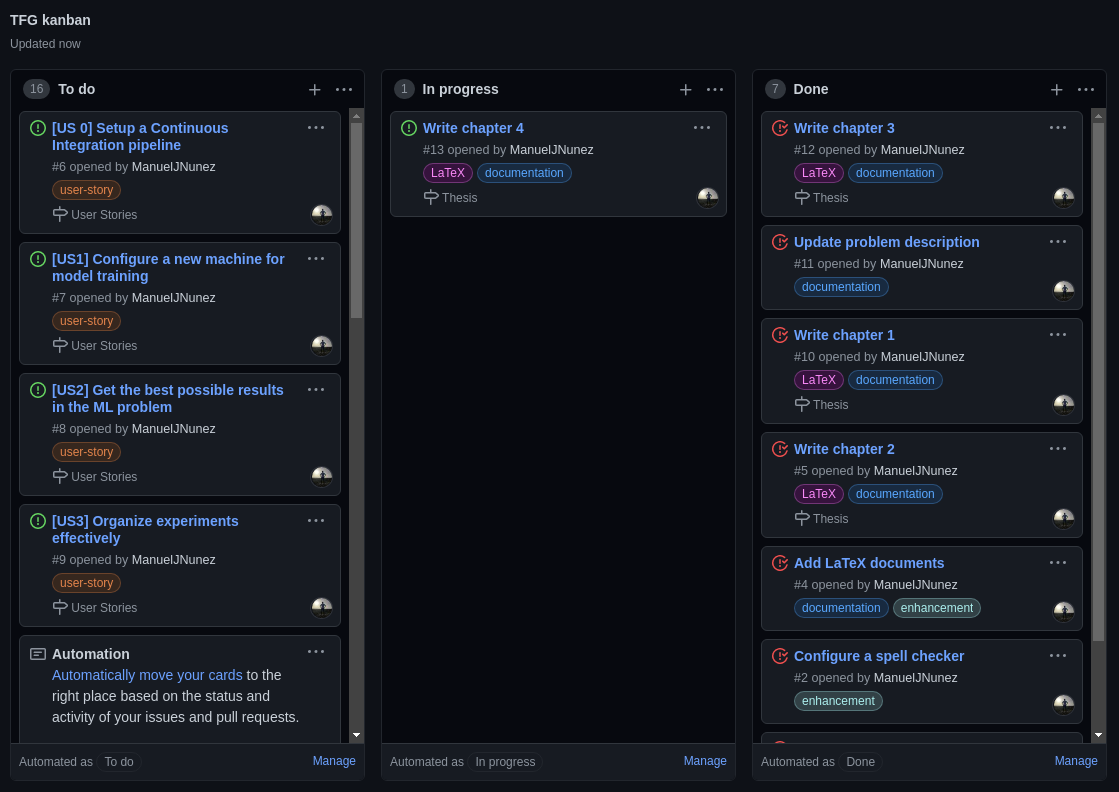
\includegraphics[scale=0.3]{imagenes/04_Planificacion/kanban.png}
	\centering
	\caption{Tablero \textit{kanban} en \textit{GitHub}. \url{https://github.com/ManuelJNunez/TFG/projects/1}}
	\label{fig:kanban}
\end{figure}

\begin{figure}[H]
  \centering
  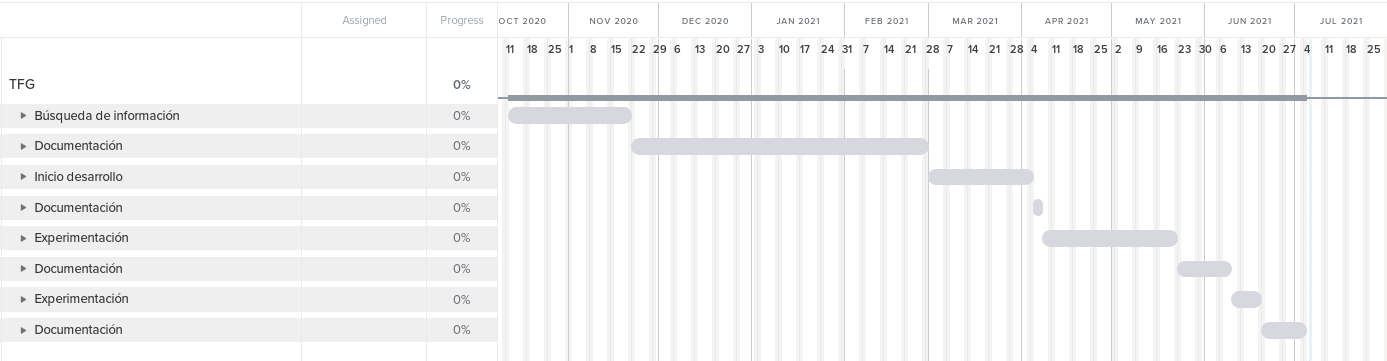
\includegraphics[width=1.\linewidth]{imagenes/04_Planificacion/gantt.png} 
  \caption{Diagrama de Gantt del proyecto.}
  \label{fig:gantt}
\end{figure}

\section{Presupuesto}

En esta Sección se va a proceder a calcular el coste del desarrollo de este proyecto, teniendo en cuenta el coste humano y material. El sueldo medio para un ingeniero de software es de aproximadamente 8,44\euro/hora, mientras que el sueldo medio de una persona que posee un doctorado es de aproximadamente 10\euro/hora\footnote{Estimación basada en la información del OTRI \cite{otri} en base a lo establecido en el BOJA número número 11 del 13 de enero de 2021 (página 281)}. En total, he dedicado 319h a este trabajo tal y como puede verse en la Figura \ref{fig:hours}. Como se puede ver en esa Figura, en el 2020 apenas le dediqué tiempo porque tenía 5 asignaturas. Sin embargo, en 2021 he podido dedicar más tiempo a este trabajo aunque tuviera prácticas de empresa y una sola asignatura.\\

\begin{figure}[H]
  \centering
  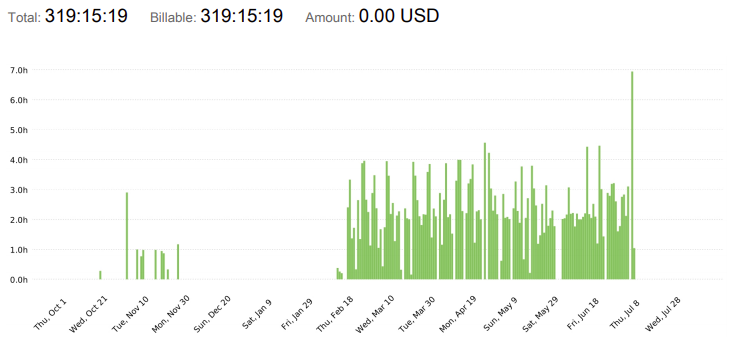
\includegraphics[width=1.\linewidth]{imagenes/04_Planificacion/hours.png} 
  \caption{Gráfico de barras y total de horas realizadas.}
  \label{fig:hours}
\end{figure}

Sobre el coste de las instancias de \textit{EC2}, no he puesto las horas de uso porque no se muestran en ninguna parte de \textit{AWS}, por tanto he puesto el coste total teniendo en cuenta los créditos con los que empecé y los que tengo ahora mismo. El coste original estaba en dólares estadounidenses, pero lo pasé a euros\footnote{Hoy día 5 de julio de 2021 el dólar estadounidense tiene un valor de 0.84\euro.}.\\

Además de todo lo anterior, he usado el nodo llamado \textit{compute-0-1} del clúster \textit{HPMoon}, el cual cuenta con el siguiente hardware y especificaciones:

\begin{itemize}
    \item Intel\textsuperscript{\textregistered} Xeon\textsuperscript{\textregistered} CPU E5-2620 v4 @ 2.10GHz (8 núcleos por procesador; 16 hebras de procesamiento en total). Su precio actual es de 449,90\euro.
    \item 32GB memoria RAM. Supongamos un precio de 200\euro\footnote{No conozco la latencia de la memoria ni la frecuencia por tanto no puedo averiguar el precio justo (supongo que usa dos módulos de 16GiB con latencia CL18 y frecuencia de 3600MHz y tipo DDR4).}.
    \item NVIDIA GeForce\textsuperscript{\textregistered} Titan Xp GPU. Descatalogada, pero su precio era de 1.349\euro\footnote{Debido a la actual falta de \textit{stock} producido por el \textit{boom} de la minería de criptomonedas, su valor no habrá variado mucho.}. Fue lanzada en el 2017.
    \item NVIDIA Tesla K40M GPU. Fue lanzada en el 2013, por tanto también está descatalogada. Algunas unidades de esta GPU que quedan en \textit{stock} tienen el valor de 796,56\euro.
    \item Una placa base con socket LGA2011-3 (compatible con el procesador anterior) y con 2 ranuras PCI Express 3.0 podría tener un valor de 160,69\euro.
    \item Además, el clúster cuenta con 15TB de capacidad de disco duro, su valor aproximado sería de 573\euro.
    \item Suponemos un chasis de servidor de 150\euro.
\end{itemize}

En total, el coste aproximado del nodo usado para entrenar modelos podría ascender actualmente a los 3679,15\euro.\\

\setlength{\tabcolsep}{10pt} % Default value: 6pt
\renewcommand{\arraystretch}{1.5} % Default value: 1

\begin{table}[H]
\centering
\begin{tabular}{ccccc}
\hline
\textbf{Tipo Coste}       & \textbf{Concepto}                                               & \textbf{Tiempo (h)} & \textbf{Coste (\euro)} & \textbf{Total (\euro)} \\ \hline
\multirow{3}{*}{Material} & \begin{tabular}[c]{@{}c@{}}Jenkins\\ (t2.medium)\end{tabular}   & -                   & 49,90              & 49,90              \\ \cline{2-5} 
               & \begin{tabular}[c]{@{}c@{}}mlflow\\ (t2.small)\end{tabular}       & -         & 34,54     & 34,54            \\ \cline{2-5} 
               & \begin{tabular}[c]{@{}c@{}}HPMoon nodo\\ compute-0-1\end{tabular} & -         & 3679,15   & 3679,15          \\ \hline
\multirow{2}{*}{Humano}   & \begin{tabular}[c]{@{}c@{}}Ingeniero\\ de software\end{tabular} & 319                 & 8,44/hora          & 2692,36            \\ \cline{2-5} 
               & Doctor                                                            & 15        & 10/hora   & 150              \\ \hline
\textbf{Total} & \textbf{}                                                         & \textbf{} & \textbf{} & \textbf{6605,95} \\ \hline
\end{tabular}
\caption{Tabla de costes}
\label{tab:costes}
\end{table}

Como se puede observar en la Tabla \ref{tab:costes}, el coste aproximado de realización de este trabajo ha sido de 6605,95\euro.
